%; whizzy chapter -dvi
% -initex iniptex -latex platex -format platex -bibtex jbibtex -fmt fmt
% 以上 whizzytex を使用する場合の設定。
 
%     Tokyo Debian Meeting resources
%     Copyright (C) 2012 Junichi Uekawa
%     Copyright (C) 2011 Nobuhiro Iwamatsu

%     This program is free software; you can redistribute it and/or modify
%     it under the terms of the GNU General Public License as published by
%     the Free Software Foundation; either version 2 of the License, or
%     (at your option) any later version.

%     This program is distributed in the hope that it will be useful,
%     but WITHOUT ANY WARRANTY; without even the implied warranty of
%     MERCHANTABILITY or FITNESS FOR A PARTICULAR PURPOSE.  See the
%     GNU General Public License for more details.

%     You should have received a copy of the GNU General Public License
%     along with this program; if not, write to the Free Software
%     Foundation, Inc., 51 Franklin St, Fifth Floor, Boston, MA  02110-1301 USA

%  preview (shell-command (concat "evince " (replace-regexp-in-string "tex$" "pdf"(buffer-file-name)) "&"))

%%ここからヘッダ開始。

\documentclass[mingoth,a4paper]{jsarticle}
\usepackage{monthlyreport}
% 日付を定義する、毎月変わります。
\newcommand{\debmtgyear}{2014}
\newcommand{\debmtgmonth}{01}
\newcommand{\debmtgdate}{18}
% started from zero:
% (let ((year 2013) (month 7)) (+ (* (- year 2005) 12) month -1))
\newcommand{\debmtgnumber}{108}

\begin{document}

\begin{titlepage}
\thispagestyle{empty}
% タイトルページ:編集必要な部分は最初のマクロに飛ばすこと

\vspace*{-2cm}
第\debmtgnumber{}回 東京エリア Debian 勉強会資料\\
\hspace*{-2cm}
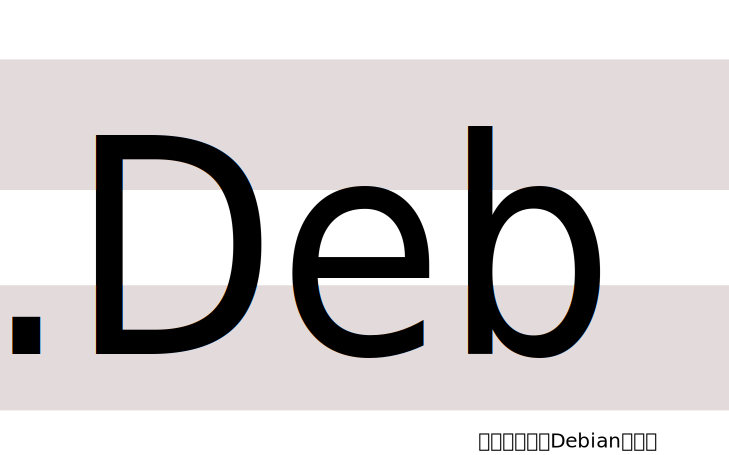
\includegraphics{image2012-natsu/dotdeb.pdf}\\
\hfill{}\debmtgyear{}年\debmtgmonth{}月\debmtgdate{}日

% ここはアップデートすること
% 全角文字にしないとフォントのサイズが合わないので注意
\rotatebox{10}{\fontsize{32}{32} {\gt 特集: Pure Blends}}\\

\vspace*{-2cm}
\hfill{}\includegraphics[height=6cm]{image200502/openlogo-nd.eps}
\end{titlepage}

\newpage

\begin{minipage}[b]{0.2\hsize}
 \definecolor{titleback}{gray}{0.9}
 \colorbox{titleback}{\rotatebox{90}{\fontsize{80}{80} {\gt デビアン勉強会} }}
\end{minipage}
\begin{minipage}[b]{0.8\hsize}
\hrule
\vspace{2mm}
\hrule
\begin{multicols}{2}
\tableofcontents
\end{multicols}
\vspace{2mm}
\hrule
\end{minipage}

\dancersection{事前課題}{野島 貴英}

今回の事前課題は以下です:
\begin{enumerate}
 \item 本日、何の作業をやるかを宣言ください。
\end{enumerate}
この課題に対して提出いただいた内容は以下です。
\begin{multicols}{2}
{\small
\begin{prework}{ 野島 貴英 }

 xmrisのパッケージ化の作業の続きをする。

\end{prework}

\begin{prework}{ 吉野(yy\_{}y\_{}ja\_{}jp) }

 (当日の東京エリアDebian勉強会で作業する内容を宣言してください という意味でしょうか)
\begin{itemize}
\item DDTSS
\item manpages-ja 続き
\end{itemize}

\end{prework}

\begin{prework}{ henrich }

fontチームのバグ潰しなど

\end{prework}

\begin{prework}{ dictoss(杉本 典充) }

FreeBSD portsのmpd5のdebパッケージ化を試みる

\end{prework}

\begin{prework}{ 野首 }

KAKASIのリリース作業を実施する。
debのnmu uploadも検討。

\end{prework}

\begin{prework}{ koedoyoshida }

最近サボっていたDDTSSでの翻訳作業を進める予定です。
\end{prework}


}
\end{multicols}

\dancersection{Debian Trivia Quiz}{野島 貴英}

ところで、みなさん Debian 関連の話題においついていますか?Debian関連の話
題はメーリングリストをよんでいると追跡できます。ただよんでいるだけではは
りあいがないので、理解度のテストをします。特に一人だけでは意味がわからな
いところもあるかも知れません。みんなで一緒に読んでみましょう。

今回の出題範囲は\url{debian-devel-announce@lists.debian.org} や \url{debian-devel@lists.debian.org}に投稿された
内容などからです。

\begin{multicols}{2}
%; whizzy-master ../debianmeetingresume201311.tex
% $B0J>e$N@_Dj$r$7$F$$$k$?$a!"$3$N%U%!%$%k$G(B M-x whizzytex $B$9$k$H!"(Bwhizzytex$B$,MxMQ$G$-$^$9!#(B
%

\santaku
{PHP$B$N%a%s%F%J%A!<%`$r#3$D$KJ,3d$9$k;v$,Ds0F$5$l$^$7$?!#J,3d$5$l$?%0%k!<%W$NL>A0$G4V0c$C$F$$$k$N$O$I$l!)(B}
{Debian PHP PECL Maintainers}
{Debian PHP PEAR Maintainers}
{Debian PHP DOCUMENT Maintainers}
{C}
{$B@5$7$/$O(B''Debian PHP Maintainers''$B$G$9!#0JA0!"(BDebian PHP Maintainers$B$O!"(BPHP$BK\BN$N%Q%C%1!<%8$b!"(BPEAR$B%b%8%e!<%k$N%Q%C%1!<%8$bN>J}%a%s%F%J%s%9$7$F$$$^$7$?!#(B}

\santaku
{Debian$B$K$D$$$F!"(BDebian Developer$B0J30$N?M$G$b9W8%$7$?$r;>$($^$7$g$&$H$$$&$3$H$G!":n$i$l$?%5%$%H$O!)(B}
{advocates.debian.org}
{contributors.debian.org}
{superstar.debian.org}
{B}
{Debian$B$K9W8%$7$?(BDebian Developer$B0J30$N?M$N%"%+%&%s%H$,(B\url{http://contributors.debian.org/}$B$K%j%9%H%"%C%W$5$l$k$h$&$K$J$j$^$7$?!#$J$*!"9W8%$K$D$$$F$N=87W$N85$O!"(B\url{https://contributors.debian.org/sources/}$B$K7G:\$5$l$F$$$k>pJs$r85$K=87W$7$F$$$k$H$N;v$G$9!#(B}

\santaku
{s390x$B%"!<%-%F%/%A%c$N%G%U%)%k%H(BC$B%3%s%Q%$%i$H$7$F$N(Bgcc$B$N%P!<%8%g%s$,JQ99$5$l$^$7$?!#$I$N%P!<%8%g%s$K$J$C$?$N$G$7$g$&!)(B}
{4.8}
{4.7}
{4.6}
{A}
{powerpc/ia64/sparc$B%"!<%-%F%/%A%c$N%G%U%)%k%H(BC$B%3%s%Q%$%i$O$^$@(Bgcc 4.6$B$N$h$&$G$9!#(BDebian$B$N<!4|%P!<%8%g%s$N(BJessie$B$G$O(Bgcc 4.6$B$O%5%]!<%HBP>]30$J$N$GAa$$$H$3$m(Bgcc 4.6$B$+$iC&5Q$9$kI,MW$,$"$j$^$9!#(B}

\santaku
{$B@hF|M-L>$J%G!<%?%Y!<%9$,%Q%C%1!<%8$H$7$FDI2C$5$l$^$7$?!#2?$H$$$&%G!<%?%Y!<%9$G$7$g$&$+!)(B}
{Maria DB}
{Percona DB}
{GDB}
{A}
{Maria DB$B$O!"(BLAMP$B%7%9%F%`$GM-L>$J(BMysql DB$B$NJL$N<BAu$G$9!#$D$$$K(BMaria DB$B%-%?!<!*:#8e$N(BMysql$B0MB8$N(BDebian$B$N%Q%C%1!<%8$NF08~$,5$$K$J$k$3$N:"$G$9!#(B}



\end{multicols}

\dancersection{最近のDebian関連のミーティング報告}{野島 貴英}

\subsection{東京エリアDebian勉強会107回目報告}

 東京エリアDebian勉強会107回目は(株)スクウェア・エニックスさんで開催されました。
5名の参加者がありました。

\begin{itemize}
\item 来年の勉強会の形式について参加者にてディスカッションをしました。\\
議論の内容:\url{http://debianmeeting.titanpad.com/debian2014?}
\item 野島さんが、Debian GNU/Hurd 2013について仮想環境による動作デモと、発表をしました。
\end{itemize}

 来年の勉強会の形式として、発表とハッカソン併用というのが有力な実施形式となりました。

 宴会は「世界のやまちゃん」にて行いました。
 

% % (query-replace-regexp "<.*?>" "")
% % (query-replace-regexp "^[	 ]\+" "")

%-------------------------------------------------------------------------------
\dancersection{Debian Pure Blend}{野島 貴英}
%-------------------------------------------------------------------------------
\index{debian-pure-blends}

\subsection{Debian Pure Blend}

 Debianに用意されている大量のパッケージをうまく使い、そのままのDebianのリポジトリを用いる事で、特定分野向けのシステムを容易にセットアップできるようにしたDebianの仕組み(考え方)となります。

 Debianパッケージに含まれるRecommends情報が利用されて、指定された特定用途のパッケージが導入される仕組みとなっています。

\subsection{用語}

 Debian Pure Blendを語る時に使われる用語を以下に載せておきます\cite{debian-pure-blends-wiki}。

\begin{table}[ht]
\begin{center}
\begin{tabular}{|l|l|p{9cm}|p{3cm}|l|}
\hline 
項番&呼び名&概要&備考 \\ \hline \hline
1 & Debian Pure Blend & そのままのDebianを用いて特定用途向けのDebianを実現 & DebiChem, Debian Edu等 \\ \hline
2 & Debian Blend & 一部のDebianでは未だ公式には採択されていないちょっとした変更を付け足し、残りはそのままのDebianを用いて特定用途向けのDebianを実現 & \\ \hline
3 & Debian Derivative & Debian派生物と日本語では言われる。目的は様々であり、Debianを元にした新しいディストリビューションを作るという点では共通。Debianをベースにしたかもしれないが、現在では大量の変更/新規機能を加えて作られているディストリビューション。& ubuntu, SteamOS \\ \hline
4 & web sentinel & \url{http://blends.debian.org}。PureBlendの種類と搭載されているパッケージ及び開発状況を載せているページ。 & \\ \hline
\end{tabular}
\label{tab:debian-blends-terms}
\caption{用語}
\end{center}
\end{table}

\subsection{利用できるPure Blend}

 現在Debian unstableで見つかったPure Blend用のパッケージの一覧を載せます。

\begin{table}[ht]
\begin{center}
\begin{tabular}{|l|l|l|p{5cm}|l|}
\hline 
項番&用途& PJ名前 & 概要&メタパッケージ名 \\ \hline \hline
1 & 子供用 & Debian Junior & 子供向けのDebianを作る & junior-* \\ \hline 
2 & 医療 & Debian Med  & 医療関係者向けのDebianを作る & med-* \\ \hline 
3 & 学校 & Debian Edu & 学校の情報教育向けのDebianを作る & education-*,debian-edu-* \\ \hline 
4 & 科学技術 & Debian Science & 科学技術向けのDebianを作る & science-* \\ \hline 
5 & マルチメディア & Debian Multimedia & マルチメディア作成関係者向けのDebianを作る & multimedia-* \\ \hline 
6 & 地理情報 & DebianGIS & 地理関係者向けのDebianを作る & gis-* \\ \hline 
7 & 化学 & Debichem & 化学関係者向けのDebianを作る & debichem-* \\ \hline 
8 & 中国語対応の一例 & Debian EzGo & 中国語に対応したDebianの1つを作る & ezgo-* \\ \hline 
\end{tabular}
\label{tab:debian-blend-package}
\caption{Debian unstableで見つかるPure Blend}
\end{center}
\end{table}

 なお、経緯を追いかけきれていないのですが、''Existing Debian Pure Blends''に記載されている他のBlendのパッケージ\cite{debian-existing-blends}を自分は見つけることができませんでした。

\subsection{使ってみる}

 早速使ってみます。ここでは、Debian Juniorを選んでみます。

\begin{description}
\item [Step 1.] debianを用意しgnome desktopを導入しておきます。
\item [Step 2.] Debian Juniorのメタパッケージの一つである、junior-gnomeを入れてみます。
\begin{commandline}
$ sudo aptitude install junior-gnome
... junior-gnome/compris/gworldclock/mathwarが導入される...
\end{commandline}
%$
\end{description}

 gnomeのメニューを見ると、gcompris/gworldclock/mathwarが新規に増えている事が分かります。

\subsection{仕組み}

 Pure Blendのパッケージは、Recommendsとしてに導入したい特定用途向けのアプリケーションが指定されています。そのため、Pure Blendのパッケージを導入すると、Recommendsに指定されたアプリケーションがまとめて導入されます。

 試しに、先の例のjunior-gnomeの依存関係を調べてみます。

\begin{commandline}
$ apt-cache depends junior-gnome
  Depends: junior-tasks
  Depends: junior-config
  Recommends: gcompris
  Recommends: gworldclock
  Recommends: mathwar
\end{commandline}
%$
 
 Recommendsとして、gcompris/gworldclock/mathwarが指定されている事がわかります。

\subsection{Pure Blend用のパッケージを作ってみる}

 Pure Blend用のパッケージを試しに作ってみます。blends-devパッケージを
導入することで、taskファイルからPure Blend用のパッケージを簡単に作る事ができます。

 ここでは、例として、ゲームのジャンルでvisual novelを選び、これらのパッケージ
を導入するようなパッケージを作成してみます。

\begin{table}[ht]
\begin{center}
\begin{tabular}{|l|l|p{5cm}|}
\hline 
項目& 内容 & 説明\\ \hline \hline
PJ名 & Debian-visualnovel & visualnovel用途向け \\ \hline 
パッケージ名 & visualnovel-* & visualnovelメタパッケージ \\ \hline 
tasksel用パッケージ & visualnovel-task & tasksel用定義ファイル \\ \hline 
\hline 
\end{tabular}
\label{tab:debian-visualnovel}
\caption{今回のPure Blendの定義}
\end{center}
\end{table}


\begin{description}
\item [Step 1.] blends-devパッケージを導入します。
\begin{commandline}
$ sudo aptitude install blend-dev
\end{commandline}
%$
\item [Step 2.] 作業ディレクトリを作り、必要なファイルをblends-devパッケージに梱包されているテンプレートをコピーして用意します。
\begin{commandline}
$ mkdir debian-visualnovel-1.0
$ cd debian-visualnovel-1.0
$ cp -a /usr/share/doc/blends-dev/examples/config .
$ cp -a /usr/share/doc/blends-dev/examples/debian .
$ cp -a /usr/share/doc/blends-dev/examples/tasks .
$ cp /usr/share/doc/blends-dev/examples/Makefile .
$ cp /usr/share/doc/blends-dev/examples/README .
\end{commandline}
%$
\item [Step 3.] コピーした各ファイルに含まれる''\_BLEND\_''の文字列を''visualnovel''に全部置き換えます。
\begin{commandline}
$ find . -type f | xargs -n 1 sed -i 's/_BLEND_/visualnovel/g'
\end{commandline}
%$
\item [Step 4.] debian/control.stubを編集します。ここで、Packageの定義として、visualnovel-tasksを必ず追加指定しておきます。また、debian/changelogも書いておきます。
\begin{commandline}
$ vi debian/control.stub
----debian/control.stubここから-------
Source: debian-visualnovel
Section: misc
Priority: extra
Maintainer: Your Name <Your mail>
Build-Depends-Indep: debhelper (>= 9),
                     blends-dev (>= 0.6.16.4)
Standards-Version: 3.9.4

Package: visualnovel-tasks
Architecture: all
Depends: tasksel
Description: Debian visualnovel for tasksel
 This package provides Debian visualnovel tasks in tasksel. 

----debian/control.stubここまで-------
$ vi debian/changelog
----debian/changelogここから------
debian-visualnovel (1.0) unstable; urgency=low

  * initial release

 -- Your Name <your@e-mail>  Mon, 13 Jan 2014 23:56:00 +0900

----debian/changelogここまで------
\end{commandline}
\item [Step 5.] tasks/task1をtasks/gameに変更し、どのパッケージを導入するか等をDepends:行に指定します。visual novelですので、onscripterと、renpy-thequestionを入れてみます。
\begin{commandline}
$ mv task/task1 task/game
$ vi task/game
--------task/gameここから----------
Task: game
Description: Debian-visual novel games_
 This metapackage will install Debian packages for use in 
 game of Debian-visualnovel

Depends: onscripter, renpy-thequestion

--------task/gameここまで----------
\end{commandline}
\item [Step 6.] パッケージを作るために必要なファイルを自動生成します。
\begin{commandline}
$ make -f debian/rules gen-orig-source
\end{commandline}
%$
\item [Step 7.] パッケージをビルドします。
\begin{commandline}
$ debuild
...visualnovel-game/visualnovel-taskパッケージが出来上がる...
\end{commandline}
%$
\end{description}

 無事visualnovel-*パッケージができました。

\subsection{おわりに}

 今回は、Debian Pure Blendの導入から作成まで説明してみました。豊富なパッケージを持つDebianならではの考え方と思います。これを機に、皆さんも何かDebian Pure Blendを作ってみませんか?

\begin{thebibliography}{0}
  \bibitem{debian-pure-blends-wiki}
    {\footnotesize{
       Debian wiki,``DebianPureBlends'',
       \url{https://wiki.debian.org/DebianPureBlends}
       }}
  \bibitem{debian-existing-blends}
    {\footnotesize{
       blends.debian.org,''Existing Debian Pure Blends'',
      \url{http://blends.debian.org/blends/ch04.html}
    }}


\end{thebibliography}


\printindex

\cleartooddpage

\vspace*{15cm}
\hrule
\vspace{2mm}
\includegraphics[width=2cm]{image200502/openlogo-nd.eps}
\noindent \Large \bf Debian 勉強会資料\\
\noindent \normalfont \debmtgyear{}年\debmtgmonth{}月\debmtgdate{}日 \hspace{5mm}  初版第1刷発行\\
\noindent \normalfont 東京エリア Debian 勉強会 (編集・印刷・発行)\\
\hrule

\end{document}
